\documentclass[conference]{IEEEtran}
\usepackage{amsmath}
\usepackage{graphicx}
\usepackage{algorithm}
\usepackage{algorithmic}
\usepackage{hyperref}

\title{Parallelized All to All Approximate Nearest Neighbors Solution}
\author{\IEEEauthorblockN{Rousomanis Georgios}
\IEEEauthorblockA{Department of Electrical and Computer Engineering\\
Aristotle University of Thessaloniki\\
Email: rousoman@ece.auth.gr}
}

\begin{document}
\maketitle

\begin{abstract}
This report presents the design and implementation of a parallelized solution to the all-to-all 
approximate nearest neighbors (A2A-ANN) problem, with an emphasis on scalability and computational 
efficiency. While the ultimate objective is to accelerate approximate similarity search in 
high-dimensional spaces where the query and candidate sets are identical ($Q = C$), the current 
work establishes a robust foundation by first solving the generalized exact k-nearest neighbors 
(k-NN) problem for the case where $Q \neq C$. The proposed implementation leverages multi-threaded 
processing and efficient matrix operations to parallelize the distance computation and top-$K$ 
selection stages. We outline the core algorithmic components, discuss strategies for memory-efficient 
execution, and lay the groundwork for extending the approach to approximate search in large-scale datasets.

\end{abstract}

\section{Introduction}
Finding the $K$ nearest neighbors (k-NN) of a point in a dataset is a fundamental operation in a wide 
range of applications, including machine learning, computer vision, information retrieval, and recommendation
systems. In its classical form, the k-NN algorithm identifies, for each query vector, the $K$ closest vectors 
in a reference dataset based on a distance metric—commonly the Euclidean distance.

This report addresses the challenge of scaling the k-NN algorithm to large datasets by parallelizing the 
computation. The ultimate goal is to solve the all-to-all approximate nearest neighbors (A2A-ANN) problem, 
where the query and candidate datasets are identical ($Q = C$), and exactness can be traded off for speed. 
This form of similarity search arises frequently in applications such as clustering, graph construction, 
and manifold learning.

As a foundational step toward the A2A-ANN goal, we begin with a parallelized implementation of the 
generalized exact k-NN problem ($Q \neq C$). This allows us to validate the parallel architecture, distance
computation kernel, and top-$K$ selection strategy in a controlled setting before introducing approximation 
techniques.

Key contributions of this work include:
\begin{itemize}
    \item A scalable, memory-efficient design for computing k-NN across two datasets using multi-threading.
    \item Efficient use of matrix operations and vector norms to accelerate distance computation.
    \item A thread-safe task management system that dynamically balances workload.
\end{itemize}

This report focuses on the high-level architecture of the implementation and its core algorithmic steps, with
emphasis on performance, memory management, and extensibility. Future work will integrate approximate search 
techniques, such as hashing or pruning heuristics, to achieve sublinear runtime for the A2A-ANN scenario.

\section{Parallelized k-Nearest Neighbors}

The core objective of the algorithm is to identify the $K$ nearest neighbors for each row in a query 
matrix $Q \in \mathbb{R}^{M \times L}$, by comparing it against a reference matrix $C \in \mathbb{R}^{N \times L}$.
Although this report initially assumes $Q \neq C$, the framework is designed to extend seamlessly to the all-to-all
setting where $Q = C$.

To measure similarity between vectors, the squared Euclidean distance is used. This choice simplifies the 
computation as it can be expressed in a form that enables precomputation and vectorized operations:

\[
D = \sqrt{C^2 - 2CQ^\top + {Q^2}^{\top}}
\]
where the square root and the exponentiation are computed element-wise.

To ensure scalability and efficient resource usage, the computation is parallelized across multiple threads. 
The strategy involves dividing the query matrix into blocks that fit within available memory constraints. 
Each block is processed independently and concurrently. The major components of this parallelization strategy 
include:

\begin{itemize}
    \item Precomputing squared norms of all vectors in both $Q$ and $C$.
    \item Using General Matrix-Matrix multiplication (GEMM) operations to compute partial distances in a 
    highly optimized manner.
    \item Assigning query blocks to worker threads through a shared task queue.
    \item Dynamically managing thread lifecycles and workload distribution to balance computation across cores.
\end{itemize}

Each thread performs the following pipeline: it pulls a query block from the task queue, computes the 
corresponding portion of the distance matrix, incorporates the precomputed norms to finalize the distance 
values, and then applies a selection algorithm to extract the top $K$ nearest neighbors for each query in 
the block. Instead of performing a full sort of distances, which is computationally expensive, the QuickSelect 
algorithm is used to identify the $K$ smallest values efficiently. This approach offers near-linear performance 
in practice and avoids unnecessary sorting overhead.

To maintain thread safety and avoid race conditions, access to the task queue is protected using mutexes and 
condition variables. A global flag is used to gracefully signal thread termination once all blocks have been
processed. Threads are initialized dynamically based on system resources, and the system waits until all threads 
have completed their assigned tasks before moving on to subsequent blocks.

Memory usage is dynamically monitored, and the size of each query block is adjusted to prevent overflows. This
adaptive approach ensures that the algorithm can scale to large datasets even on systems with limited memory.

The correctness of the algorithm was verified by generating multiple random datasets and comparing its output 
against the results produced by MATLAB's built-in knnsearch function. Distance values and corresponding neighbor 
indices were cross-validated to ensure consistency and accuracy.

Overall, the methodology combines vectorized numerical operations, concurrent task execution, and intelligent 
memory management to enable fast and scalable nearest neighbor computation. This foundation is well-suited for 
future extensions into approximate search and all-to-all nearest neighbor graph construction.

\section{k-Nearest Neighbors Benchmarks}

We evaluated the performance of the exact k-NN implementation by varying the number of threads used during 
execution. Benchmarks were conducted using the MNIST dataset on a 4-core system running Ubuntu 22.04 LTS. 
The results are presented in Fig.~\ref{fig:knn_benchmarks}.

The plot illustrates how query throughput (measured in queries per second) increases with the number of threads,
peaking when the number of threads matches the number of physical CPU cores. Beyond this point, performance 
begins to degrade due to overheads associated with thread contention and context switching.

The blue solid line shows the performance of our algorithm when the number of application-level threads corresponds
to the x-axis value, while the number of OpenBLAS threads is fixed at one. The red dashed line, in contrast, 
represents performance when our algorithm runs with a single thread while OpenBLAS utilizes all 4 cores internally.

It is evident that the best performance is achieved when our parallelized implementation manages the 4 threads 
directly, resulting in a speedup of approximately 1.8× compared to relying solely on OpenBLAS multithreading. 
This improvement is attributed to more efficient workload distribution and reduced overhead in the application's 
threading model.

\begin{figure}
\centering
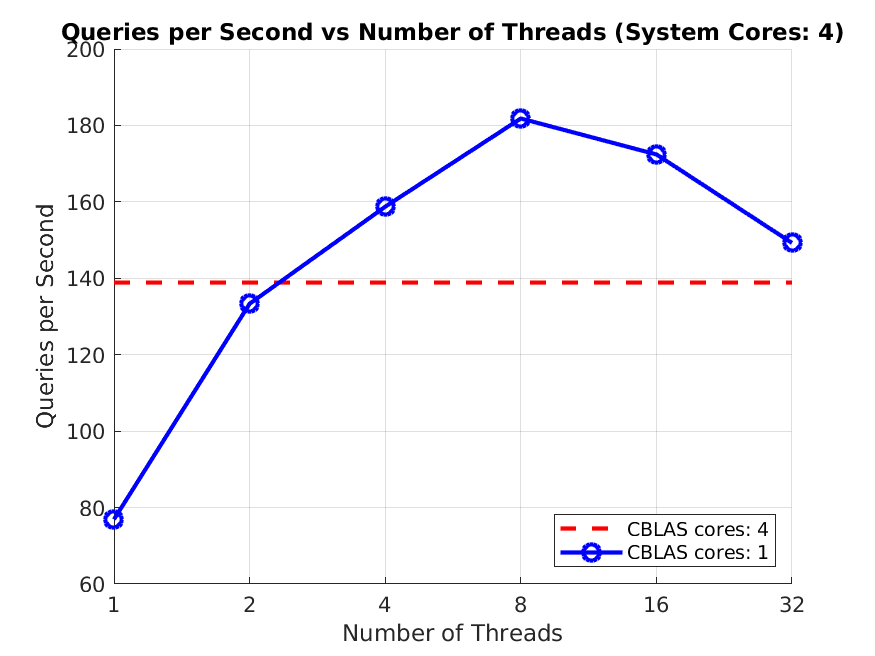
\includegraphics[width=1\linewidth]{figures/knn_benchmarks.png}
\caption{Performance comparison of different threading configurations for exact k-NN on the MNIST dataset.}
\label{fig:knn_benchmarks}
\end{figure}

\bibliographystyle{IEEEtran}
\bibliography{references}
\end{document}
